\section{Physikalische Grundlagen}

\subsection{Funktionsweise eines Lasers}


Der Laser stellt eines der wichtigsten Werkzeuge der Experimentalphysik dar. Es gibt viele
verschiedene Arten von Lasern, die grundsätzliche Funktionsweise ist jedoch immer ähnlich. Man
benötigt zunächst ein aktives Medium, in dem optische Übergänge stattfinden, die zur Emission von
Photonen führen. Außerdem benötigt man eine optische Pumpe, die eine Besetzungsinversion im Medium
erzeugt, wodurch sich mehr Atome im Zustand höherer Energie befinden. Dazu benötigt man mindestens
drei Zustände: Einen Grundzustand, von dem aus die Elektronen in einen ersten angeregten Zustand
gepumpt werden, welcher mit möglichst kurzer Lebensdauer in einen weiteren angeregten Zustand etwas
niedriger Energie fällt, der eine möglichst lange Lebensdauer besitzt. Dies verhindert, dass die
Photonen des Laserlichts direkt wieder absorbiert werden und Atome im niedrigen Zustand
anheben. Zusätzlich benötigt man einen Resonator, der Photonen mit einer bestimmten Energie und
Impuls in den Laser zurückkoppelt. Diese Photonen regen dann Atome dazu an, in den niedrigeren
Zustand zu fallen und dabei ein Photon mit gleicher Energie und Impuls zu emittieren. Das führt zu
dem gewollten monochromatischen und kohärenten Licht.
Wenn mehrere verschiedene Übergänge zur Verfügung stehen, wird die Wellenlänge des Lasers durch die
minimalsten Verluste sowie die Wirkungsquerschnitte der Übergänge bestimmt. Die Verluste sind
hierbei vor allem vom Resonator beeinflusst, zum Beispiel über die Reflektivität der Spiegel.



\subsection{Stabilitätskriterium des Resonators}


Ein Resonator ist stabil, wenn ein Strahl auch nach beliebig vielen Reflexionen den Resonator nicht
verlässt.
Mit Hilfe von Matrizenoptik lässt sich dafür das Stabilitätskriterium eines Resonators
ableiten:

\begin{equation}
0\leq g_1 \cdot g_2 \leq 1
\end{equation}

wobei $g_1=(1-\frac{L}{R_1})$ und $g_2=(1-\frac{L}{R_2})$ mit den Krümmungsradien der Spiegel
$R_{1/2}$ und dem Abstand der Spiegel L. In diesem Versuch verwenden wir hauptsächlich einen
hemisphärischen Resonator mit einem Spiegel mit einem Krümmungsradius von 100\,mm, für die
Frequenzverdopplung wird jedoch ein sphärischer Resonator benötigt mit einem zweiten Spiegel mit
einem Krümmungsradius von 150\,mm.
In Abb.~\ref{img:stabkrit} sind die Verläufe von $g_1 \cdot g_2$ als Funktion des Abstands der
Spiegel dargestellt. Daraus ergibt sich für den hemisphärischen Resonator ein stabiler Zustand für
einen Abstand bis 100\,mm und für den sphärischen Resonator zusätzlich von 150\,mm bis 250\,mm.

\begin{figure}[H]
\begin{center}
  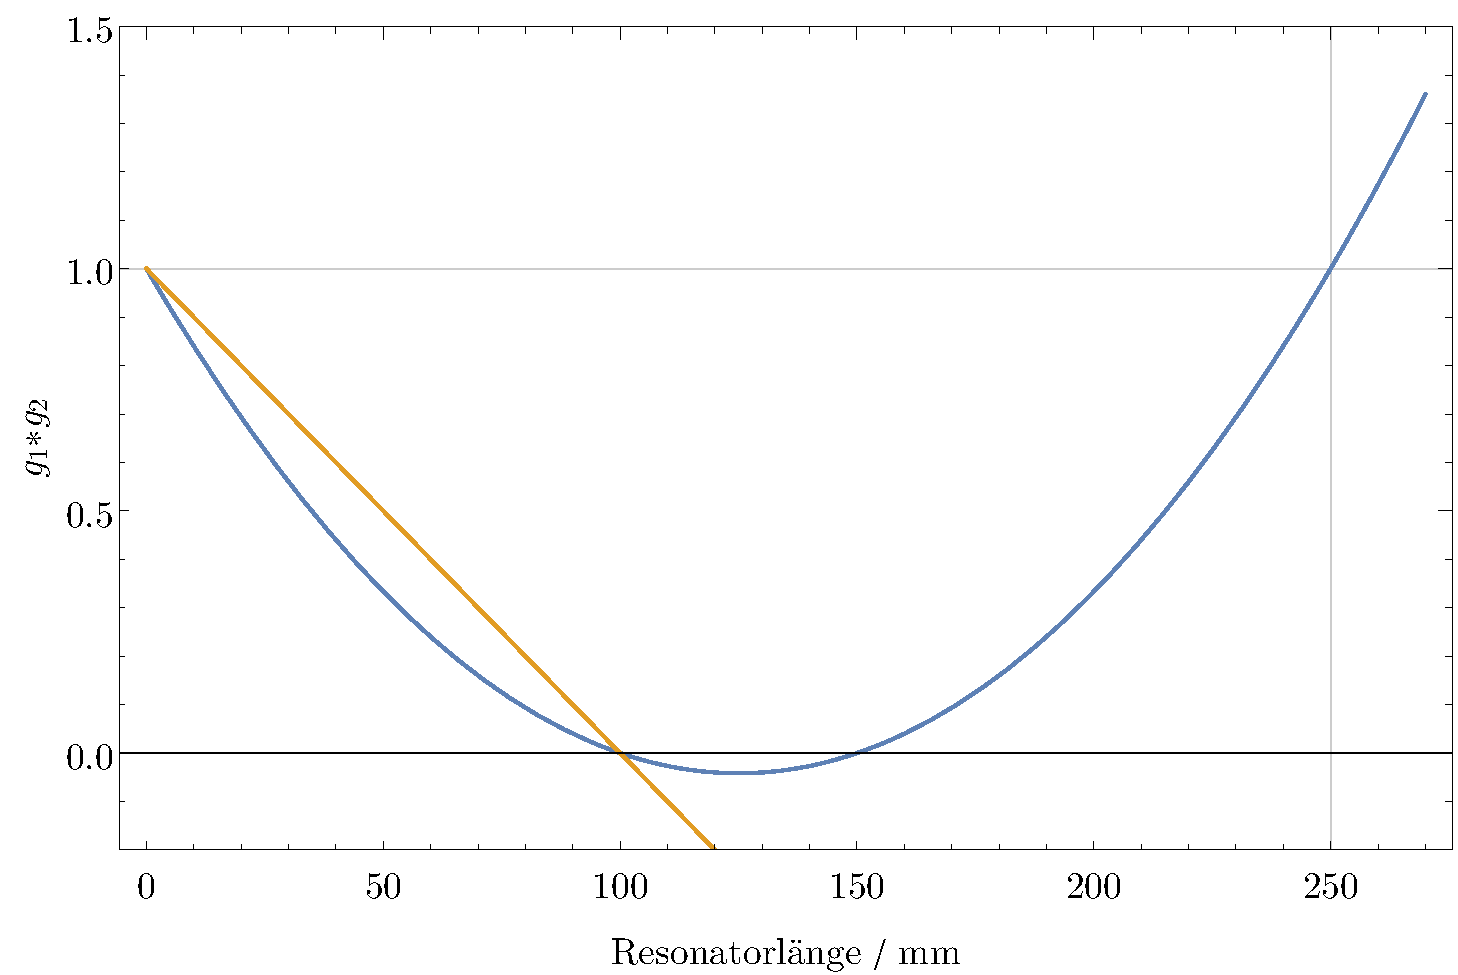
\includegraphics[width=.7\textwidth]{Stabkrit1.pdf}
  \caption{Darstellung des Stabilitätskriteriums für unsere verwendeten Laserresonatoren als
  Funktion des Abstands der Spiegel. Für $g_1\cdot g_2$ zwischen 0 und 1 ist der Resonator stabil.}
  \label{img:stabkrit}
\end{center}
\end{figure}


\subsection{Eigenschaften des Pr:YLF-Lasers}

2. What are the specific characteristics of a Pr:YLF laser, i.e., why is it interesting to use a Pr:YLF
laser compared to other solid state lasers? In your answer, also make a comparison of the Pr:YLF
laser with the ruby laser and the Nd:YAG laser.

\begin{figure}[H]
\begin{center}
  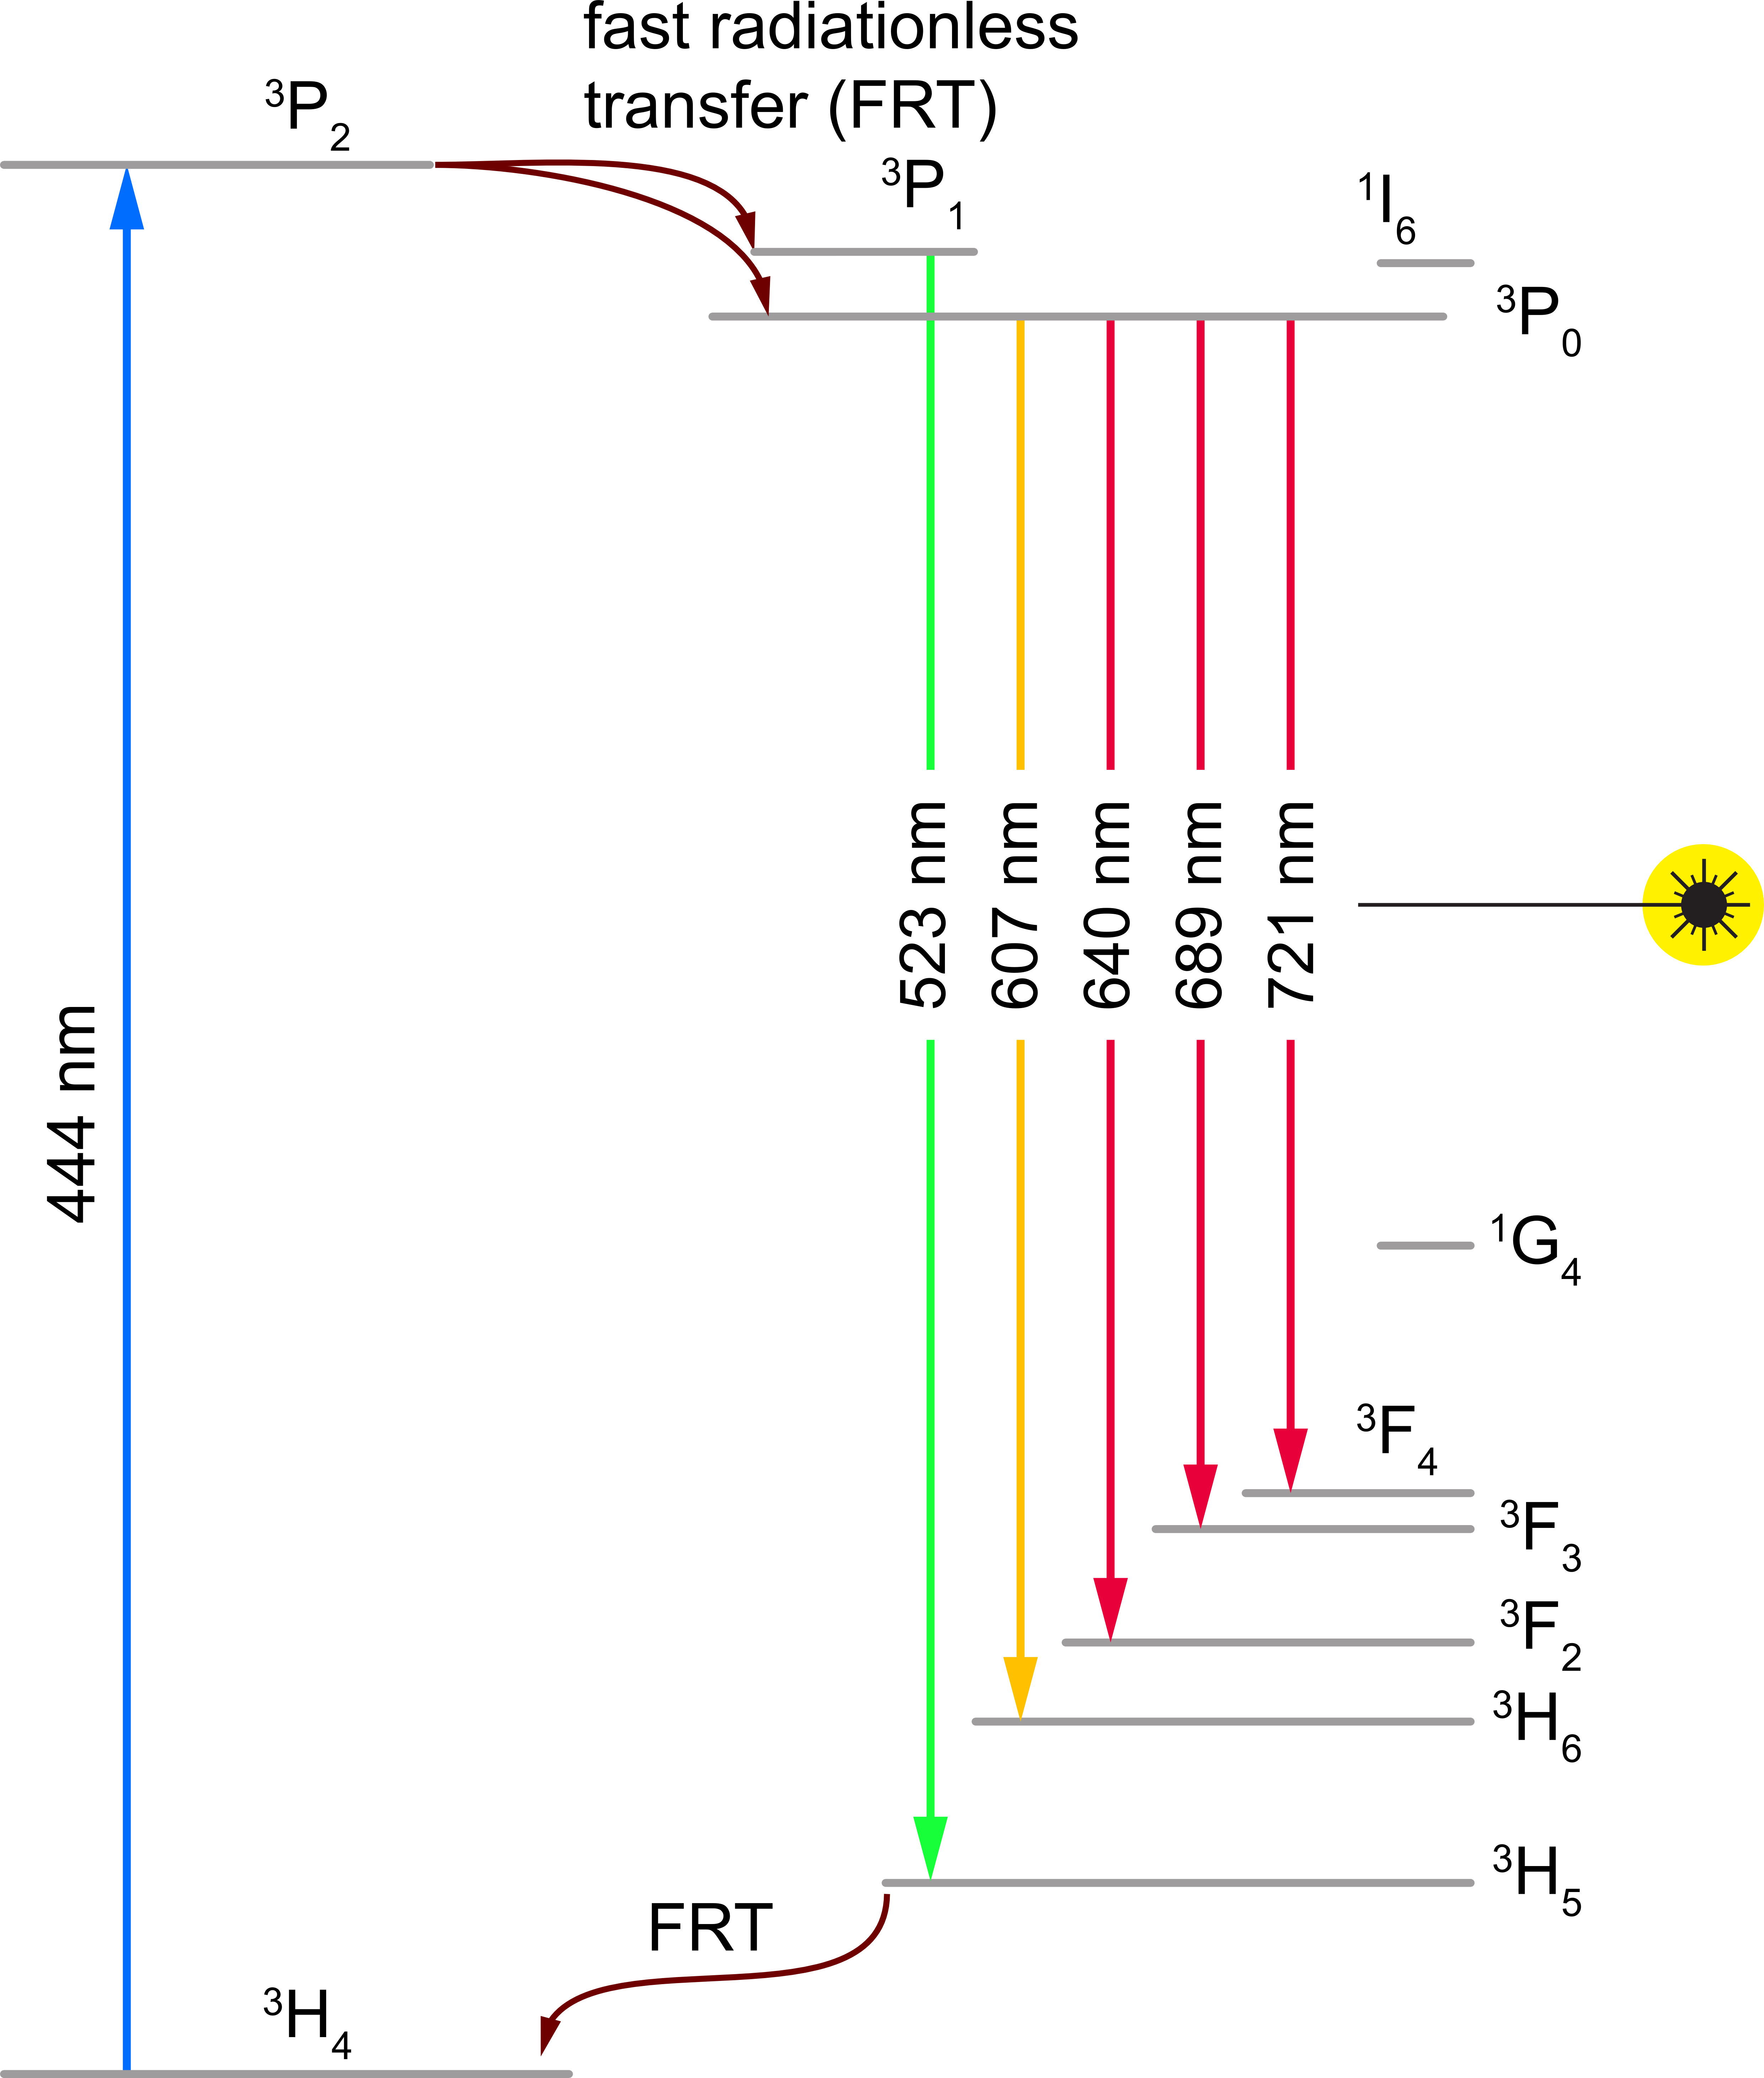
\includegraphics[width=.45\textwidth]{TermschemaPr3+.png}
  \caption{Termschema von Pr$^{3+}$ und relevante Übergänge für den Laserbetrieb
  \cite{Versuchsanleitung}.}
  \label{img:Termschema}
\end{center}
\end{figure}

\subsection{Wellenlängenselektion}


3. Compare the working principles of a birefringent tuner with those of a Littrow prism.


\subsection{Frequenzverdopplung}

4. How does second harmonic generation work and why does it have a low
efficiency?



\subsection{Laserschutzbrillen}

\begin{figure}[H]
\begin{center}
  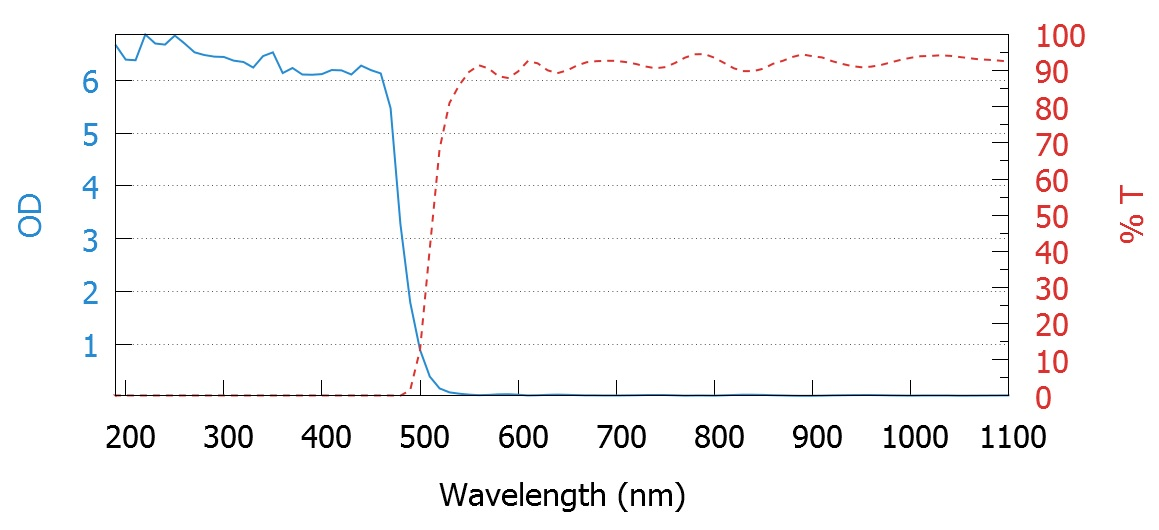
\includegraphics[width=.7\textwidth]{Schutzbrillen.png}
  \caption{Absorptions- (blau)  und Transmissionsspektrum (rot) der im Versuch
  verwendeten Laserschutzbrillen \cite{Versuchsanleitung}.}
  \label{img:Schutzbrillen}
\end{center}
\end{figure}

Abb.~\ref{img:Schutzbrillen} zeigt das Absorptions- und Transmissionsspektrum der
Laserschutzbrillen, die im Versuch verwendet werden.
Strahlung mit Wellenlängen unter 450\,nm wird um einem Faktor von mehr als $10^6$ abgeschwächt und
der starke blaue Pumplaser bei 444\,nm damit fast vollständig blockiert.
Bei Wellenlängen über 500\,nm beginnt eine signifikante Transparenz und über 550\,nm gelangt mehr
als 90\,\% des Lichts durch die Schutzbrillen,
so dass die Linien des Pr:YLF-Lasers beobachtet werden können.

